\chapter{Implementation and Experimental Results}
\label{ch:implementation}

Henceforth, we evaluate out system experimentally and compare the results with the theoretical analysis.
We begin this chapter by a description of the implementation in \Cref{sec:implementation}.
Then, we move on to describing our experimental setup in \Cref{sec:experimental-setup}.
Finally, \Cref{sec:evaluation} presents our experimental results and our evaluation.
Our experiment primarily focuses on the consensus duration and the throughput.


\section{Implementation}
\label{sec:implementation}

The prototype implementation can be found on GitHub\footnote{\url{https://github.com/kc1212/consensus-thesis-code}}.
It is written in the event driven paradigm, using the Python programming language\footnote{\url{https://www.python.org/}} and
the Twisted\footnote{\url{https://twistedmatrix.com/}} library for networking.

The structure of the implementation is primarily made up of three modules---\texttt{acs}, \texttt{trustchain} and \texttt{node}.
\texttt{acs}, as its name suggests, implements ACS.
ACS uses erasure code in one of its subprotocols (reliable broadcast).
Thus we use the liberasurecode\footnote{\url{https://github.com/openstack/liberasurecode}} library for its Reed-Solomon error correcting code functionality.
An implementation detail is that liberasurecode cannot create more than 32 code blocks\footnote{
  The 32 code blocks limitation is hardcoded in the source file, see
  \url{https://github.com/openstack/liberasurecode/blob/0794b31c623e4cede76d66be730719d24debcca9/include/erasurecode/erasurecode.h\#L35}
}, we discuss the effect of this in~\Cref{sec:experimental-setup}.
The \texttt{acs} module provides a small interface to the caller to start and stop the consensus process and also retrieve results.
The \texttt{trustchain} module implements the Extended TrustChain data structure.
It also provides the essential algorithm necessary to interact with Extended TrustChain such as 
$\textsf{new\_tx}(\cdot)$, $\textsf{new\_cp}(\cdot)$, $\textsf{agreed\_fragment}(\cdot)$ and so on.
Since this is a prototype implementation, we only store the data structure in memory and not on disk.
Finally, the \texttt{node} module ties everything together.
It implements the the consensus protocol, the transaction protocol and the validation protocol.

Every node keeps a persistent TCP connection with every other node.
This creates a fully connected network for our experiment.
It is certainly not ideal in real world scenarios where nodes may have limited resources (e.g. sockets).
But as a prototype, it is sufficient to run a network of over a thousand nodes and experiment with it.

Finally, the cryptography primitives we use are SHA256 for hash functions and Ed25519 for digital signatures.
Both of which are provided by libnacl~\footnote{\url{https://pypi.python.org/pypi/libnacl}}.


\section{Experimental Setup}
\label{sec:experimental-setup}

The the goal of the experiment is to run the three protocols---consensus protocol,
transaction protocol and validation protocol---simultaneously and analyse the throughput, consensus duration and other related metrics.
We investigate these properties under the following four parameters.
\begin{enumerate}
  \item The transaction rate $r_{\text{tx}}$ per node. This is not comparable to the others because it is fixed at 2 TX/s.
        Nevertheless, it is a good value because, as we show later,
        it hits a bottleneck in extreme cases which helps us understand the limitations of our design.
  \item The number of facilitators $n \in \{ 12, 16, \dots, 32\}$.
        Unfortunately, the maximum $n$ is 32 because the limitation in liberasurecode mentioned in \Cref{sec:implementation}.
  \item The population size $N \in \{200, \dots, 1200\}$.
        $N$ stops at 1200 is due to our physical setup, which we describe next.
  \item The two modes of transaction.
        The first mode or the ideal mode is that nodes only transact with their immediate neighbour. 
        This minimises the data volume per validated transaction because agreed fragment can be cached.
        The second mode is in the other extreme, where every transaction is with a random node out of the $N$ nodes in the system,
        thus the agreed fragment is unlikely to be cached.
\end{enumerate}

The experiment is run on the DAS-5 (The Distributed ASCI Supercomputer 5\footnote{\url{https://www.cs.vu.nl/das5/}}).
From now on, we use "machines" to refer to DAS-5 nodes and nodes to refer to a running instance in our system.
On DAS-5 we use up to 30 machine, for each machine we use 40 nodes.
This gives us the aforementioned 1200 number.
With this setup, we cannot run more nodes because the every machine only has 65535 ports available (minus the reserved ones).
But 40 nodes each need 1200 TCP connections which is 48000 TCP connections per machine and that is inching close to the limit.
While it is possible to have many more TCP connections per machine,
but it requires additional network interface which is something we do not control on the DAS-5.

To coordinate nodes on many different machine,
we employ a discovery server to inform every node the IP addresses and port numbers of every other node.
It is only run before the experiment and is not used during the experiment.


\section{Communication cost for a round}

\begin{figure}[tb]
  \centering
  \makebox[\linewidth][c]{%
    \begin{subfigure}[b]{.7\textwidth}
      \includegraphics[width=1.0\textwidth]{neighbour-fixed/round-communication-cost-vs-population}
      \caption{Transactions are with fixed neighbours}
      \label{fig:consensus-comms-fixed}
    \end{subfigure}%
    \begin{subfigure}[b]{0.7\textwidth}
      \includegraphics[width=1.0\textwidth]{neighbour-random/round-communication-cost-vs-population}
      \caption{Transactions are with random neighbours}
      \label{fig:consensus-comms-random}
    \end{subfigure}%
  }
\end{figure}

\Cref{fig:consensus-comms} show the relationship between communication cost and population.
These most important aspect is that these results show a linear increase.
This reinforces our analytical result in~\Cref{sec:acs-complexity}.
Further, note that regardless of whether the transactions are performed with a random neighbour or with a fixed neighbour,
the magnitude of the communication cost are similar.
Both peak at about $1.4 \times 10^{10}$ bytes.
This is expected because the consensus protocol is decoupled from the transaction protocol.

We are also interested in how communication costs translate to time.
Hence, for the same experiment we use duration in seconds on the vertical axis instead of communication cost and plot the~\Cref{fig:consensus-duration}
These show a similar trend as the communication cost graphs.
Hence our assumption (from~\Cref{sec:acs-time-complexity}) that for every unit of communication there is some fixed overhead is valid.

\section{Communication Cost for Transaction and Validation}

\begin{figure}[h]
  \centering
  \begin{subfigure}{\textwidth}
    \includegraphics[width=\textwidth]{neighbour-fixed/tx-communication-cost-vs-population}
    \caption{Transactions are with fixed neighbours}
    \label{fig:tx-comms-fixed}
  \end{subfigure}

  \begin{subfigure}{\textwidth}
    \includegraphics[width=\textwidth]{neighbour-random/tx-communication-cost-vs-population}
    \caption{Transactions are with random neighbours}
    \label{fig:tx-comms-random}
  \end{subfigure}
  \caption{Communication cost per verified transaction}
  \label{fig:tx-comms}
\end{figure}

Recall that in~\Cref{sec:communication-cost-for-tx} we argued that the communication cost per verified transaction is of $O(N)$.
To verify the argument, we plot the relationship between the communication cost and population size in~\Cref{fig:tx-comms}.
Again, we observe a linear relationship, which verified the argument.

However, note that there is a large difference in communication cost between the two modes of transaction.
When transacting with only one neighbour, the communication cost is low because only one agreed fragment needs to be communicated for every round in order to validate all transactions of that round.
This is because agreed fragments are cached.
On the other hand,
if every node is transacting with a random node, then it is likely the case that one agreed fragment needs to be communicated for every transaction.
Hence the communication cost we see in~\Cref{fig:tx-comms-random} is much higher than in~\Cref{fig:tx-comms-fixed}.

It is interesting to note that some fluctuations exist in the graphs.
This is likely due to the way how the communication cost are recorded.
We maintain the total amount of data sent and received in a few variables.
On every message that is sent or received, we increment the relevent variable by the size of the message.
However, it is infeasible to log the values every time a message is sent or received as there is simply too much data for our build server to hold.
Therefore we only log every 5 seconds.
This does not always align with the time when a round finishes, thus some of the data may not represent reality accurately.
%  TODO this can be fixed

\section{Global Throughput}
The global throughput results are shown in~\Cref{fig:global-throughput}.
Clearly, the throughput has a linear relationship with the population size.
This result is a strong indication of the horizontal scalability which we aimed to achieve.
It also verified our analytical result in~\Cref{sec:global-throughput}.

More interestingly, is the magnitude in throughput, 
and the difference in magnitude between the two modes of transaction.
Firstly, recall that we fixed our $r_\text{tx}$ to 2, but how is it possible to have nearly 9000 transactions per second for 1200 nodes (which is about 7.5 transactions per second)?
This is due to the way validated transactions are calculated.
Transactions are between two parties, hence if every node makes two transactions per seoncd,
every node also expects to receive two transactions per second.
Hence, for every node, the TX blocks are created at 4 per second.
Every TX block must be validated.
So everyone sends 4 validation requests per second and also receives 4 per second.
Thus during one second 8 validations are performed.
The difference in magnitude is caused by the caching mechanism mentioned earlier.
If an agreed fragment needs to be transmitted to validating every transaction then it puts a toll on the network infrastructure.
The low transaction rate in~\Cref{fig:global-throughput-random} is caused by fact that the network infrastructure cannot keep up with our demand.
We demonstrate this issue from a different angle in the next section.

\begin{figure}[h]
  \centering
  \begin{subfigure}{\textwidth}
    \includegraphics[width=\textwidth]{neighbour-fixed/throughput-vs-population}
    \label{fig:global-throughput-fixed}
  \end{subfigure}

  \begin{subfigure}{\textwidth}
    \includegraphics[width=\textwidth]{neighbour-random/throughput-vs-population}
    \label{fig:global-throughput-random}
  \end{subfigure}
  \caption{Global throughput}
  \label{fig:global-throughput}
\end{figure}



\section{Backlog}

TODO

\begin{figure}[h]
  \centering
  \begin{subfigure}{\textwidth}
    \includegraphics[width=\textwidth]{neighbour-fixed/timeseries}
  \end{subfigure}

  \begin{subfigure}{\textwidth}
    \includegraphics[width=\textwidth]{neighbour-random/timeseries}
  \end{subfigure}
\end{figure}